%%%%%%%%%%%%%%%%%%%%%%%%%%%%%%%%%%%%%%%%%
% Stylish Article
% LaTeX Template
% Version 2.1 (1/10/15)
%
% This template has been downloaded from:
% http://www.LaTeXTemplates.com
%
% Original author:
% Mathias Legrand (legrand.mathias@gmail.com) 
% With extensive modifications by:
% Vel (vel@latextemplates.com)
%
% License:
% CC BY-NC-SA 3.0 (http://creativecommons.org/licenses/by-nc-sa/3.0/)
%
%%%%%%%%%%%%%%%%%%%%%%%%%%%%%%%%%%%%%%%%%

%----------------------------------------------------------------------------------------
%	PACKAGES AND OTHER DOCUMENT CONFIGURATIONS
%----------------------------------------------------------------------------------------

\documentclass[fleqn,10pt]{SelfArx} % Document font size and equations flushed left

\usepackage[english]{babel} % Specify a different language here - english by default
\usepackage{lipsum} % Required to insert dummy text. To be removed otherwise
\setlength{\columnsep}{0.55cm} % Distance between the two columns of text
\setlength{\fboxrule}{0.75pt} % Width of the border around the abstract
\definecolor{color1}{RGB}{0,0,90} % Color of the article title and sections
\definecolor{color2}{RGB}{0,20,20} % Color of the boxes behind the abstract and headings
\usepackage{hyperref} % Required for hyperlinks
\hypersetup{hidelinks,colorlinks,breaklinks=true,urlcolor=color2,citecolor=color1,linkcolor=color1,bookmarksopen=false,pdftitle={Title},pdfauthor={Author}}
\usepackage{algorithm}
\usepackage{algorithmic}
\usepackage{multirow}
\usepackage{amsmath}
\usepackage{amssymb}
\def\Plus{\texttt{+}}	
\def\Minus{\texttt{-}} 
\usepackage{amsfonts}
\usepackage{alltt}
\usepackage{url}
\usepackage{relsize}
\usepackage{adjustbox}
\usepackage{graphicx}



%----------------------------------------------------------------------------------------
%	ARTICLE INFORMATION
%----------------------------------------------------------------------------------------

\JournalInfo{Computer Science\\School of Informatics, Computing, and Engineering\\Indiana University, Bloomington, IN, USA} % Journal information
\Archive{Datamining B565 Fall 2017}  % Additional notes (e.g. copyright, DOI, review/research article)

\PaperTitle{Kaggle Competitions:\\ \ Spooky Author Identification\\ \ Statoil/C-CORE Iceberg Classifier Challenge} % Article title

\Authors{Ashay Sawant\textsuperscript{1}*, Samanvitha Pradhan\textsuperscript{1}*, John Stein\textsuperscript{2}*} % Authors
\affiliation{\textsuperscript{1}\textit{Data Science, School of Informatics, Computing, and Engineering, Indiana University, Bloomington, IN, USA}} % Author affiliation
\affiliation{*\textbf{Corresponding author}: ahsawant@iu.edu} % Corresponding author
\affiliation{*\textbf{Corresponding author}: sspradha@iu.edu} % Corresponding author
\affiliation{\textsuperscript{2}\textit{Computer Science, School of Informatics, Computing, and Engineering, Indiana University, Bloomington, IN, USA}} % Author affiliation
\affiliation{*\textbf{Corresponding author}: jodstein@iu.edu} % Corresponding author

\Keywords{NLP --- Natural Language Processing --- SAR --- Image Recognition} % Keywords - if you don't want any simply remove all the text between the curly brackets
\newcommand{\keywordname}{Keywords} % Defines the keywords heading name
\usepackage{abstract}

%----------------------------------------------------------------------------------------
%	Executive Summary
%----------------------------------------------------------------------------------------

\Abstract{\textbf{Executive Summary} 
	This report summarizes two Datamining projects undertaken by the authors.  The first project attempts to classify `scattered pages' from works of fiction written by Edgar Allan Poe, HP Lovecraft, and Mary Wollstonecraft Shelley according to their author.  Various approaches were explored, including TBD (Samanvitha).  The best-performing approach was achieved by TBD, with a Log Loss of TBD.  The second project attempts to classify Synthetic Aperture Radar images according to whether the image has captured an iceberg or not.  Again, various approaches were explored including Logistic Regression using custom features, TBD (Ashay).  The best-performing approach was achieved by Logistic Regression using custom features, with a Log Loss of 0.3682 (TBD, Ashay update this if you do better!).
	}


\begin{document}

\renewcommand{\abstractname}{}  
\renewcommand{\absnamepos}{} 

\flushbottom % Makes all text pages the same height
\maketitle % Print the title and abstract box
\tableofcontents % Print the contents section
\thispagestyle{empty} % Removes page numbering from the first page

%----------------------------------------------------------------------------------------
%	ARTICLE CONTENTS
%----------------------------------------------------------------------------------------

\section{Introduction}
The two projects presented herein (Spooky Author Identification and Iceberg Classifier Challenge) are the results of the combined efforts of the authors to meet the corresponding challenges published by Kaggle. \cite{kaggle-author} \cite{kaggle-ice}  Kaggle.com is a site dedicated to the Data Science community where entities can post problems and challenges to be taken on by Data Science academics and enthusiasts.  Readers can find more details on each of these challenges at Kaggle's website \footnote{\url{https://www.kaggle.com/}} in the Competitions section.

Datamining (DM) has three broad areas of application: answering questions, exploring and discovering relationships, and annotation.  Kaggle competitions, including those described in this paper, are a convenient way for an entity with a requirement in one of these application spaces to draw from a large community of willing problem solvers to find effective and efficient solutions to satisfy their requirement.  Spooky Author Identification is considered a `Playground Competition', meaning the underlying motivation is to encourage increased participation in the Kaggle community and potentially spur innovative advances in to standing challenges in Natural Language Processing.  In the case of Iceberg Classification, the underlying requirement is for Statoil to accurately and efficiently identify icebergs that could threaten their sea-based natural resources operations.  In both cases, DM presents an opportunity to discover useful relationships between written word and their author or between SAR imagery and the target being imaged, to enable classification accuracy and efficiency well beyond human performance.

\subsection{Author Identification}
TBD - Samanvitha please complete this section.
What is the problem to be solved?  What is the data? How is goodness quantified?  This should not be too technical, but we can say, for example, given three authors $A = \{a_1, a_2, a_3\}$ and selections of their individiually corresponding works $S_{a_1}, S_{a_2}, S_{a_3}$,  we are constructing a probability  mass function $f$ over $A$ that is applied to a text $t$ written by one of the authors, but unlabled:
\begin{equation}
f(A|t,S) = \{p_{a_1}, p_{a_2}, p_{a_3}\}
\end{equation}

A text is simply a passage from one of the author's works:
\begin{quote}
Once upon a midnight dreary, while I pondered, weak and weary, Over many a quaint and curious volume of forgotten lore—While I nodded, nearly napping, suddenly there came a tapping, As of some one gently rapping, rapping at my chamber door.“’Tis some visitor,” I muttered, “tapping at my chamber door— Only this and nothing more.”
\end{quote}
from Edgar Allen Poe's, \textit{The Raven}.  You must find out whether it's only prose -- and how much of the original structure is maintained.  Likely you will not take in text directly -- so this must be described.


\subsection{Statoi/C-CORE Iceberg Classifier Challenge}

The Iceberg Classifier Challenge is to accurately classify whether a Synthetic Aperture Radar (SAR) image contains an iceberg or something that is not an iceberg, which makes it a binary classification problem.  The data provided includes an $75 \times 75$ image that represents horizontally polarized backscatter intensity (\texttt{band\_1}), a $75 \times 75$ image that represents vertically polarized backscatter intensity (\texttt{band\_2}), and the angle of incidence between Earth-normal and the transmit beam (\texttt{inc\_angle}).  Training data also contains the class label (\texttt{is\_iceberg}).  The classifier is to calculate the probability that the image contains an iceberg (1) or not (0).  Kaggle evaluates the goodness of the classifier using Log Loss, shown below.

$$LL = - \frac{1}{N} \sum_{i=1}^N t_i log(y(x_i)) + (1-t_i) log(1-y(x_i))$$

The best classifiers will have Log Loss scores near zero.  Receiver Operator Characteristics (ROC) was also used to evaluate the True Positive vs False Positive behavior of the classifier.  High-performing classifier will have ROC curves that resemble a step function and with an area under the curve (AUC) near 1.0.  \footnote{ROC finds its origins in World War 2 as radar operators were evaluated on their ability to distinguish real targets from false targets and clutter. \cite{Lusted1217}}


\section{Datamining}

\begin{itemize}[noitemsep]

\item What is DM?  DM seeks to inform decision making by answering questions about, exploring or discovering relationships in, or providing annotation of data.

\item What does it yield?  DM yields information that is not possible or practical to directly observe, based on data that is practical to observe.  This information may be predicted trends in human behavior, perceived relationships or clusters within high-dimension data, or a prediction of future events.  In all cases, the yielded information is deemed valuable to someone who is then enabled to make decisions based on that information.

\item What are the general steps?  

\begin{itemize}
	
	\item The first (and most difficult) step in DM is developing the problem statement: What decision or action is the DM effort required to inform or enable, and what must the DM effort yield in order to satisfy that requirement?
	
	\item The second step is data acquisition.  Acquisition of data is non-trivial.  It can be difficult, expensive, and in some cases even prohibited or restricted by law.  Therefore, the miner must be intentional about pursuing the acquisition of data that is both needed (from the problem statement) and available, whether by manual observation, survey, or automated sensing/recording.
	
	\item The third (and most time consuming) step in data-mining is data pre-processing.  The data must be analyzed, including identifying unknown, missing, or outlier records, examining attributes and their domains, and visualizing the data for first-order behaviors, trends, and distributions.  The data must then be integrated and/or cleaned, including dealing with unknown, missing, or bad data, enriching the data from other sources, and/or transforming the data to work better in the algorithm.
	
	\item The fourth step is to actually mine the data (i.e. answer questions, explore or discover relationships, or annotate).  The methodology, assumptions, models, and parameters of how the mining is performed can depend on the objective, the data itself, and the miner themselves.
	
	\item The fifth and final step in DM is to interpret the output of the mining step and either validate that it meets the stated objective/requirement of the problem statement, or determine that changes to the pre-processing or mining steps are warranted and start again with a modified approach.

\end{itemize}

\item What is clustering \textit{vs.} classification?  Classification refers to the task of predicting the label of some unobserved target attribute given a set of observed attributes for some record.  The label is generally a single member of a finite list of possible labels.  Clustering refers to the task of identifying or discovering relationships among data.  In other words, are there properties or measures for which subsets of data can be interpreted as similar or dissimilar in a meaningful way?  Clustering aims to discover these `clumps' or similar data as well as the properties or measurements from which the similarity can be determined.  It is useful to think of Classification as a supervised learning task because it is notionally possible to produce a training set with labeled records, and Clustering as an unsupervised learning task because the number and meaning of the discovered clusters is not known apriori (if they were, they could be labeled and it would be called Classification).

\item What is a loss function? A loss function is a function which attempts to assign a real value to some undesirable property of an intermediate outcome during the mining step.  This value (known as cost or loss) may represent error, variance, or bias of a model, clustering, or classifier.  The actual value of loss is usually not meaningful.  Instead, the goal is generally to minimize the loss over some parameter or variable during an optimization step.

\end{itemize}


\subsection{Data Preprossing}

\begin{itemize}[noitemsep]

\item What are the steps, and what challenges does each present?  The first step in data preprocessing is data analysis.  Data analysis can include examining histograms, bar/pair-plots, frequency tables, etc.  The goal is to get familiar with the data attributes and their domains, frequency of values, trends and distributions, and first-order behaviors.  From the analysis, the two primary remaining tasks are selection and modification.  Selection (i.e. sampling and attribute selection) refers to deciding which subset or records and/or which subset of attributes for each record to use for the mining task.  Modification (i.e. aggregation, dimensionality reduction, discretization, and transformation) refers to changing existing, creating new, or transforming, attributes and their values.

\begin{itemize}
	
	\item Sampling refers to choosing a subset of the total data from which to develop the analysis technique - often because working on the entire dataset would result in more resource investment than it would improve the performance of the technique.  The challenge with sampling is that, especially for high-dimensionality data, the data data can quickly become sparse, resulting in a greater potential for over-fitting due to the small data size and high dimensionality (degrees of freedom).
	
	\item Attribute Selection refers to selecting which attributes to include in the analysis and which to exclude, based on some preliminary analysis.  Manual attribute selection (or de-selection) is challenging because humans can only perceive date in two, three, or perhaps four dimensions.  One can only reasonably expect to act on the most obvious of attribute properties without impacting the analysis in unexpected ways.
	
	\item Aggregation refers to manually grouping several attributes or attribute values together, preferably while preserving some higher-level relationship among those being grouped.  Aggregation can be relatively straightforward in some cases, but in other cases it can be very difficult to group attributes or values in a way that recognizes the essential common property of its members.
	
	\item Dimensionality Reduction refers to the creation of fewer new attributes which are combinations of the many old attributes.  Two common methods include Principal Component Analysis (PCA) and Neural Networks.  The primary challenge with dimensionality reduction is that the meaning of the original attributes are all but lost as the data are mapped to the new, reduced feature space.
	
	\item Discretization refers to the assignment of values from a continous-valued attributes into one of finite-many bins.
	
	\item Transformation refers to the mapping of old attribute values to new attribute values - generally reversible.
\end{itemize}
Finally, data with unknown, erroneous, or missing values must be handled.  Some of these handling techniques may be implemented in the mining algorithm(s) themselves, but some may be performed prior to the mining step.  Unknown/missing data handling is more challenging for some algorithms (i.e. regression) than it is for others (i.e. decision trees).  Some algorithms need each record to have good data, or they will simply not work.  Other algorithms can be made to handle unknown/missing data in a reliable way and achieve good performance.  Still other algorithms can operate on records having missing data with no extra effort.  The primary challenge, especially for high-dimensionality data, is that the impact of the handling technique can be different for every attribute, and must be understood and chosen carefully.

\item What is the general load (time, space, \$) for preprocessing?  Computationally, preprocessing may consume $O(n)$ or $O(n log m)$ time where $n$ is the number of records to process and $m$ may be search steps if matching, inclusion, or sorting operations are required.  Preprocessing may consume anywhere from constant space to $O(n)$ space, if the records are processed one at a time and stored back into their original location, or copies are made.  Practically speaking, preprocessing can consume upwards of 80\% of the labor hours, and therefore ~80\% of the funding, of the overall DM effort.  That is because it is the most human-intensive step of the process.  Automation of the preprocessing step, although possible, is of limited benefit if the DM problems vary significantly in size, scope, data representation, purpose, etc.  The ability to predict the preprocessing impacts of data across problem spaces is indeed an analytics problem unto itself.

\end{itemize}

\subsection{Mining, Interpretation, and Action}

\paragraph{Top Ten Algorithms in DM}
Below is a brief overview of the top 10 algorithms in DM. \cite{Wu:2007:TAD:1327434.1327436}

\begin{itemize}
	\item{\textbf{C4.5:}} C4.5 is an algorithm that can be used for decisions trees or rulesets. For trees, tt essentially builds a decision tree by recursively splitting the data on attributes until the data is fully explained by the tree.  It then prunes the tree by calculating a binomial error estimate at each of the leaves, and comparing that with the error that would be introduced by collapsing to the parent node, and repeating until complete.  For rulesets, it similarly generates rules representing every complete path through the notional unpruned tree (i.e. the rules generated fully explain the data).  Then, C4.5 discards conditions in the generated rules to minimize the binomial error estimate using hill-climing techniques.  Finally, in both cases, a default rule is created in case data do not satisfy any of the remaining rules.
	\item{\textbf{K-Means:}} K-Means naively assigns K centroids to the space shared by the data, and then assigns each data point to the centroid that is closest (according to some distance function).  Next, the algorithm computes new locations for the existing centroids based on that data points that are assigned to them.  Then the data points are reassigned, if they are now closer to a different centroid.  The process continues until convergence, which is guaranteed, and the centroids are taken to be the resulting clusters.
	\item{\textbf{Support Vector Machines:}} SVMs attempt to find some hyperplan that fully seperates the data into their proper classes, so that the hyperplane can be used to estimate classes for future data.  It chooses the hyperplane with the maximum distance from the nearest data.  Many times the data is not linearly separable.  Two primary approaches have been adopted in such cases: (a) the introduction of a slack variable can be used to assign a penalty to any hyperplane that incorrectly classifies some of the training data, and the task becomes to minimize that penalty, and (b) the data can be kernelized, or mapped onto a new space, which is linearly separable using traditional SVM. 
	\item{\textbf{Apriori:}} The Apriori algorithm was developed to efficiently find frequent sets.  It relies on the truth that if an item is not frequent in some set, then any superset containing that item is also not frequent in that set.  Starting with singletons, candidate frequent subsets are generated from frequent subsets of lower cardinality, and then eliminated, thereby eliminating the need to check for frequency on subsets that could not be frequent.
	\item{\textbf{Expectation Maximization:}} EM is a more general case of K-Means.  For any probabilistic model, the parameters for that model are initialized to some starting value, and then the model is then used to cluster the training data.  In many cases, the clustering is performed via soft-assignment, meaning each data point is assigned a probability of belonging to each cluster.  Based on the new clustering, parameters for the model are recalculated to best fit the data assigned to each.  Then the data are reassigned, and the process repeats until convergence (to some threshold) is achieved.
	\item{\textbf{Page Rank:}} Page Rank is intended to find relative importance of hub nodes in a complex network, commonly applied to web pages on the Internet.  Essentially each page is assigned a rank value that is the sum of all contributions of pages that link to it.  Each incoming contribution is the contributing page's rank value divided by the number of outgoing links it has.  In this way, the highest page ranks are achieved when a page has many links to it that come from pages with high rank and few outgoing links.
	\item{\textbf{Adaboost:}} Adaboost is a type of ensemble learning algorithm that uses voting to create strong learners from multiple weak learners.  Essentially, the algorithm picks a single (best) learner by which to classify training (labled) data.  It then assigns a weight to each training sample, lower for those that were correctly classified and higher for those that were not.  It then selects a new (best) feature and similarly redistributes the weight to misclassified examples.  After the last weak learner is used, each learner is then weighted according to the weighted error they would have using the final weights on the misclassified examples in each learner.  The final weighted weak learners represents the new stronger ensemble learner.
	\item{\textbf{K Nearest Neighbors:}} KNN is a relatively simple algorithm that finds the K nearest neighbors to each data points and either clusters that data point according to whichever cluster was most frequent in the neighbors, or clusters that data point according to a weighted (by distance) vote from the nearest neighbors.
	\item{\textbf{Naive Bayes:}} Naive Bayes classifiers essentially assume that all the features belonging to a dataset are independent of each other, given the class.  Essentially, joint probability distributions are created (rather efficiently using the chain rule, due to the independence assumption) to provide a purely probabilistic estimate of class, based on the training data.
	\item{\textbf{Classification and Regression Trees (CART):}} CART is an umbrella term encompassing several variations on building trees for use with categorical or real-valued data.  In general, they work by building binary classification trees using intelligent selection criteria for choosing attributes to split on (such as information gain or the Gini impurity), and then perform pruning of the resulting tree (or stopping criteria) by minimizing a loss which contains a complexity penalty element and a misclassification (or error, in the real-valued case) element.
\end{itemize}

Despite DM's many benefits, the algorithms do not solve problems or tell users what to do.  It is up to the human Dataminer to clearly understand the problem space, define what they need from the DM solution, exercise the DM process, interpret and validate the results and limitations of the results, and then use the results to inform their action.

New types of problems in DM include finding more stable decision-tree algorithms, decomposition of complex models into ensembles of simpler models, and improvement in feature selection techniques. \cite{Wu:2007:TAD:1327434.1327436} Additional (albeit tangential) topics related to DM include security/privacy implications of DM, the convergence of DM and Internet of Things (IoT), and novel applications of DM.






%------------------------------------------------
%
%  Author Identication
%   
%------------------------------------------------
\section{Author Idenfication: Full Problem Description}
\begin{itemize}[noitemsep]
\item Define problem
\item Formally describe problem--inputs, outputs, training and testing method
\end{itemize}

%\begin{figure*}[ht]\centering % Using \begin{figure*} makes the figure take up the entire width of the page
%\includegraphics[width=\linewidth]{view}
%\caption{You can span in the width of the page if you need to.}
%\label{fig:view}
%\end{figure*}

\lipsum[4] % Dummy text

\begin{equation}
\cos^3 \theta =\frac{1}{4}\cos\theta+\frac{3}{4}\cos 3\theta
\label{eq:refname2}
\end{equation}

\lipsum[5] % Dummy text


\subsection{Data Analysis}
\begin{itemize}[noitemsep]
\item Describe the data in full detail--from its raw form to the transformation
\item Provide summary statistics and relationships
\end{itemize}

\lipsum[6] % Dummy text

\subsection{Methods}
\begin{itemize}[noitemsep]
\item Discuss the algorithm you've chosen, \textit{e.g.}, why you chose it
\item Provide some background material on your method that shows you are well-acquianted with it
\item Challenges to your method
\item What software and hardware did you use, packages, \textit{etc.}
\item Final structure of data after preprocessing
\item Present training and testing as some combination of text and visualizations
\end{itemize}
%\begin{figure}[ht]\centering
%\includegraphics[width=\linewidth]{results}
%\caption{Any illustration should first says what it is.  Then describe the axes.  What is important in the graph.  There should be a title too.}
%\label{fig:results}
%\end{figure}
Algorithm\,\ref{alg:1} shows an extended $k$-means.

\begin{algorithm}
\caption{This is a caption for the algorithm.  $k$-means* over $\Delta$}
\label{alg:1}
\begin{algorithmic}[1]
\STATE{\ {\bf INPUT} data $\Delta$, blocks k, distance $\textbf{d}:\Delta^2 \rightarrow \Re_{\geq 0}$}
\STATE{\ {\bf OUTPUT} centroids $C_1,\ldots,C_l$}
\STATE \%\% assume that a centroid is a pair $(v,X)$
\STATE \%\% $v\in \Re^m$ and (a possibly empty) $ X\subseteq \Delta$
\STATE \%\% heap $ H \subseteq \Delta$
\STATE{\ randomly construct k centroids $\mathbf{\mathsf{C}}^0 = \{C_1^0, C_2^0,\ldots,C_k^0\}$}
\STATE{\ $i \leftarrow 0$ }
\STATE \%\% $\Delta_{HE}$ represents HE data, $\Delta = \Delta_{HE} +  \Delta_{LE}$
\STATE{\ $\Delta_{HE} \leftarrow \Delta$}
\REPEAT
\FOR {$\mathbf{x} \in \Delta_{HE}$}
\FOR { $C_j^i \in \mathbf{\mathsf{C^i}}$}
\STATE \%\% assign data to centroid/heap that is nearest
\STATE \%\% $\sigma \Rightarrow d$
\STATE $C_j^i.H.insert(\mathbf{x},d)$, where min$\{ \textbf{d}(\mathbf{x}, C_j^i.v)\}$
\ENDFOR
\ENDFOR
\STATE{\ $\Delta^\prime \leftarrow \emptyset$}
\FOR {$C_j^i \in \mathbf{\mathsf{C^i}}$}
\STATE \%\% recalculate centroid as average of over $C.H$
\STATE $C_j^{i+1}.v \leftarrow  \sum\nolimits_{\mathbf{x} \in C_j^i.X} (\mathbf{x}/|C_j^i.X|) $
\STATE{\ $\Delta^\prime \leftarrow C_j^i.H.flush(\sigma)$}
\STATE{\ $ \mathbf{\mathsf{C^{i+1}}} \xleftarrow{\cup} \{ C_j^{i+1}\} $}
\ENDFOR
\STATE{\ $i \leftarrow i+1$ }
\STATE{\ $\Delta_{HE} \leftarrow \Delta^\prime$}
\UNTIL{threshold on $\mathbf{\mathsf{C^{i-1}}}$}
\end{algorithmic}
\end{algorithm}


%Reference to Figure \ref{fig:results}.

%------------------------------------------------

\subsection{Results}
\begin{itemize}[noitemsep]
\item Dispassionately describe your results both quantified and qualified
\item Do you deem this successful
\item What do the results suggest
\item What were challenges
\end{itemize}
Remember, we're interested in the journey, so simply because an approach failed doesn't mean failure if you discuss the failure!
\subsection{Summary and Future Work}
\begin{itemize}[noitemsep]
\item Briefly summarize project and outcome
\item What would you do differently in the future?
\end{itemize}

\lipsum[10] % Dummy text
\section{Iceberg: Full Problem Description}

Statoil, an energy company with oil and natural gas operations based largely in the Norwegian Continental Shelf region, has an operational need to track the presence of icebergs that may present a threat to the safety and efficiency of those operations. \cite{statoil} The company has therefore posed the following iceberg classification problem to the data science community.  Statoil partners with C-CORE (a Canadian R\&D corporation) to obtain access to Synthetic Aperture Radar (SAR) imagery data from the Sentinel-1 satellite constellation, and the challenge is to classify the object in each image as an iceberg or non-iceberg (presumably a ship, which is not likely to pose a threat to operations). A labeled training set (1604 records) and an unlabeled test set (8424 records) is provided, and the task is to classify each image as containing an iceberg (\texttt{is\_iceberg}=1) or not (\texttt{is\_iceberg}=0). \cite{kaggle-ice}

\subsection{Data Analysis}
Each record contains three components (besides an identifier):

\begin{itemize}
	\item \texttt{band\_1} - 75$\times$75 pixel image representing horizontally-polarized backscatter intensity from the horizontally-polarized C-band radar transmission
	\item \texttt{band\_2} - 75$\times$75 pixel image representing vertically-polarized backscatter intensity from the horizontally-polarized C-band radar transmission
	\item \texttt{inc\_angle} - angle of incidence (between the transmission path and Earth-normal at the target object)
\end{itemize}

\paragraph{Initial Analysis} Some simple statistical analysis on the image data reveals that maximum and mean values in both bands are meaningful contributors to the classification task, as shown in Figure \ref{max-mean-separable}.

\begin{figure}[ht]
	\centering
	\begin{minipage}{0.24\textwidth}
		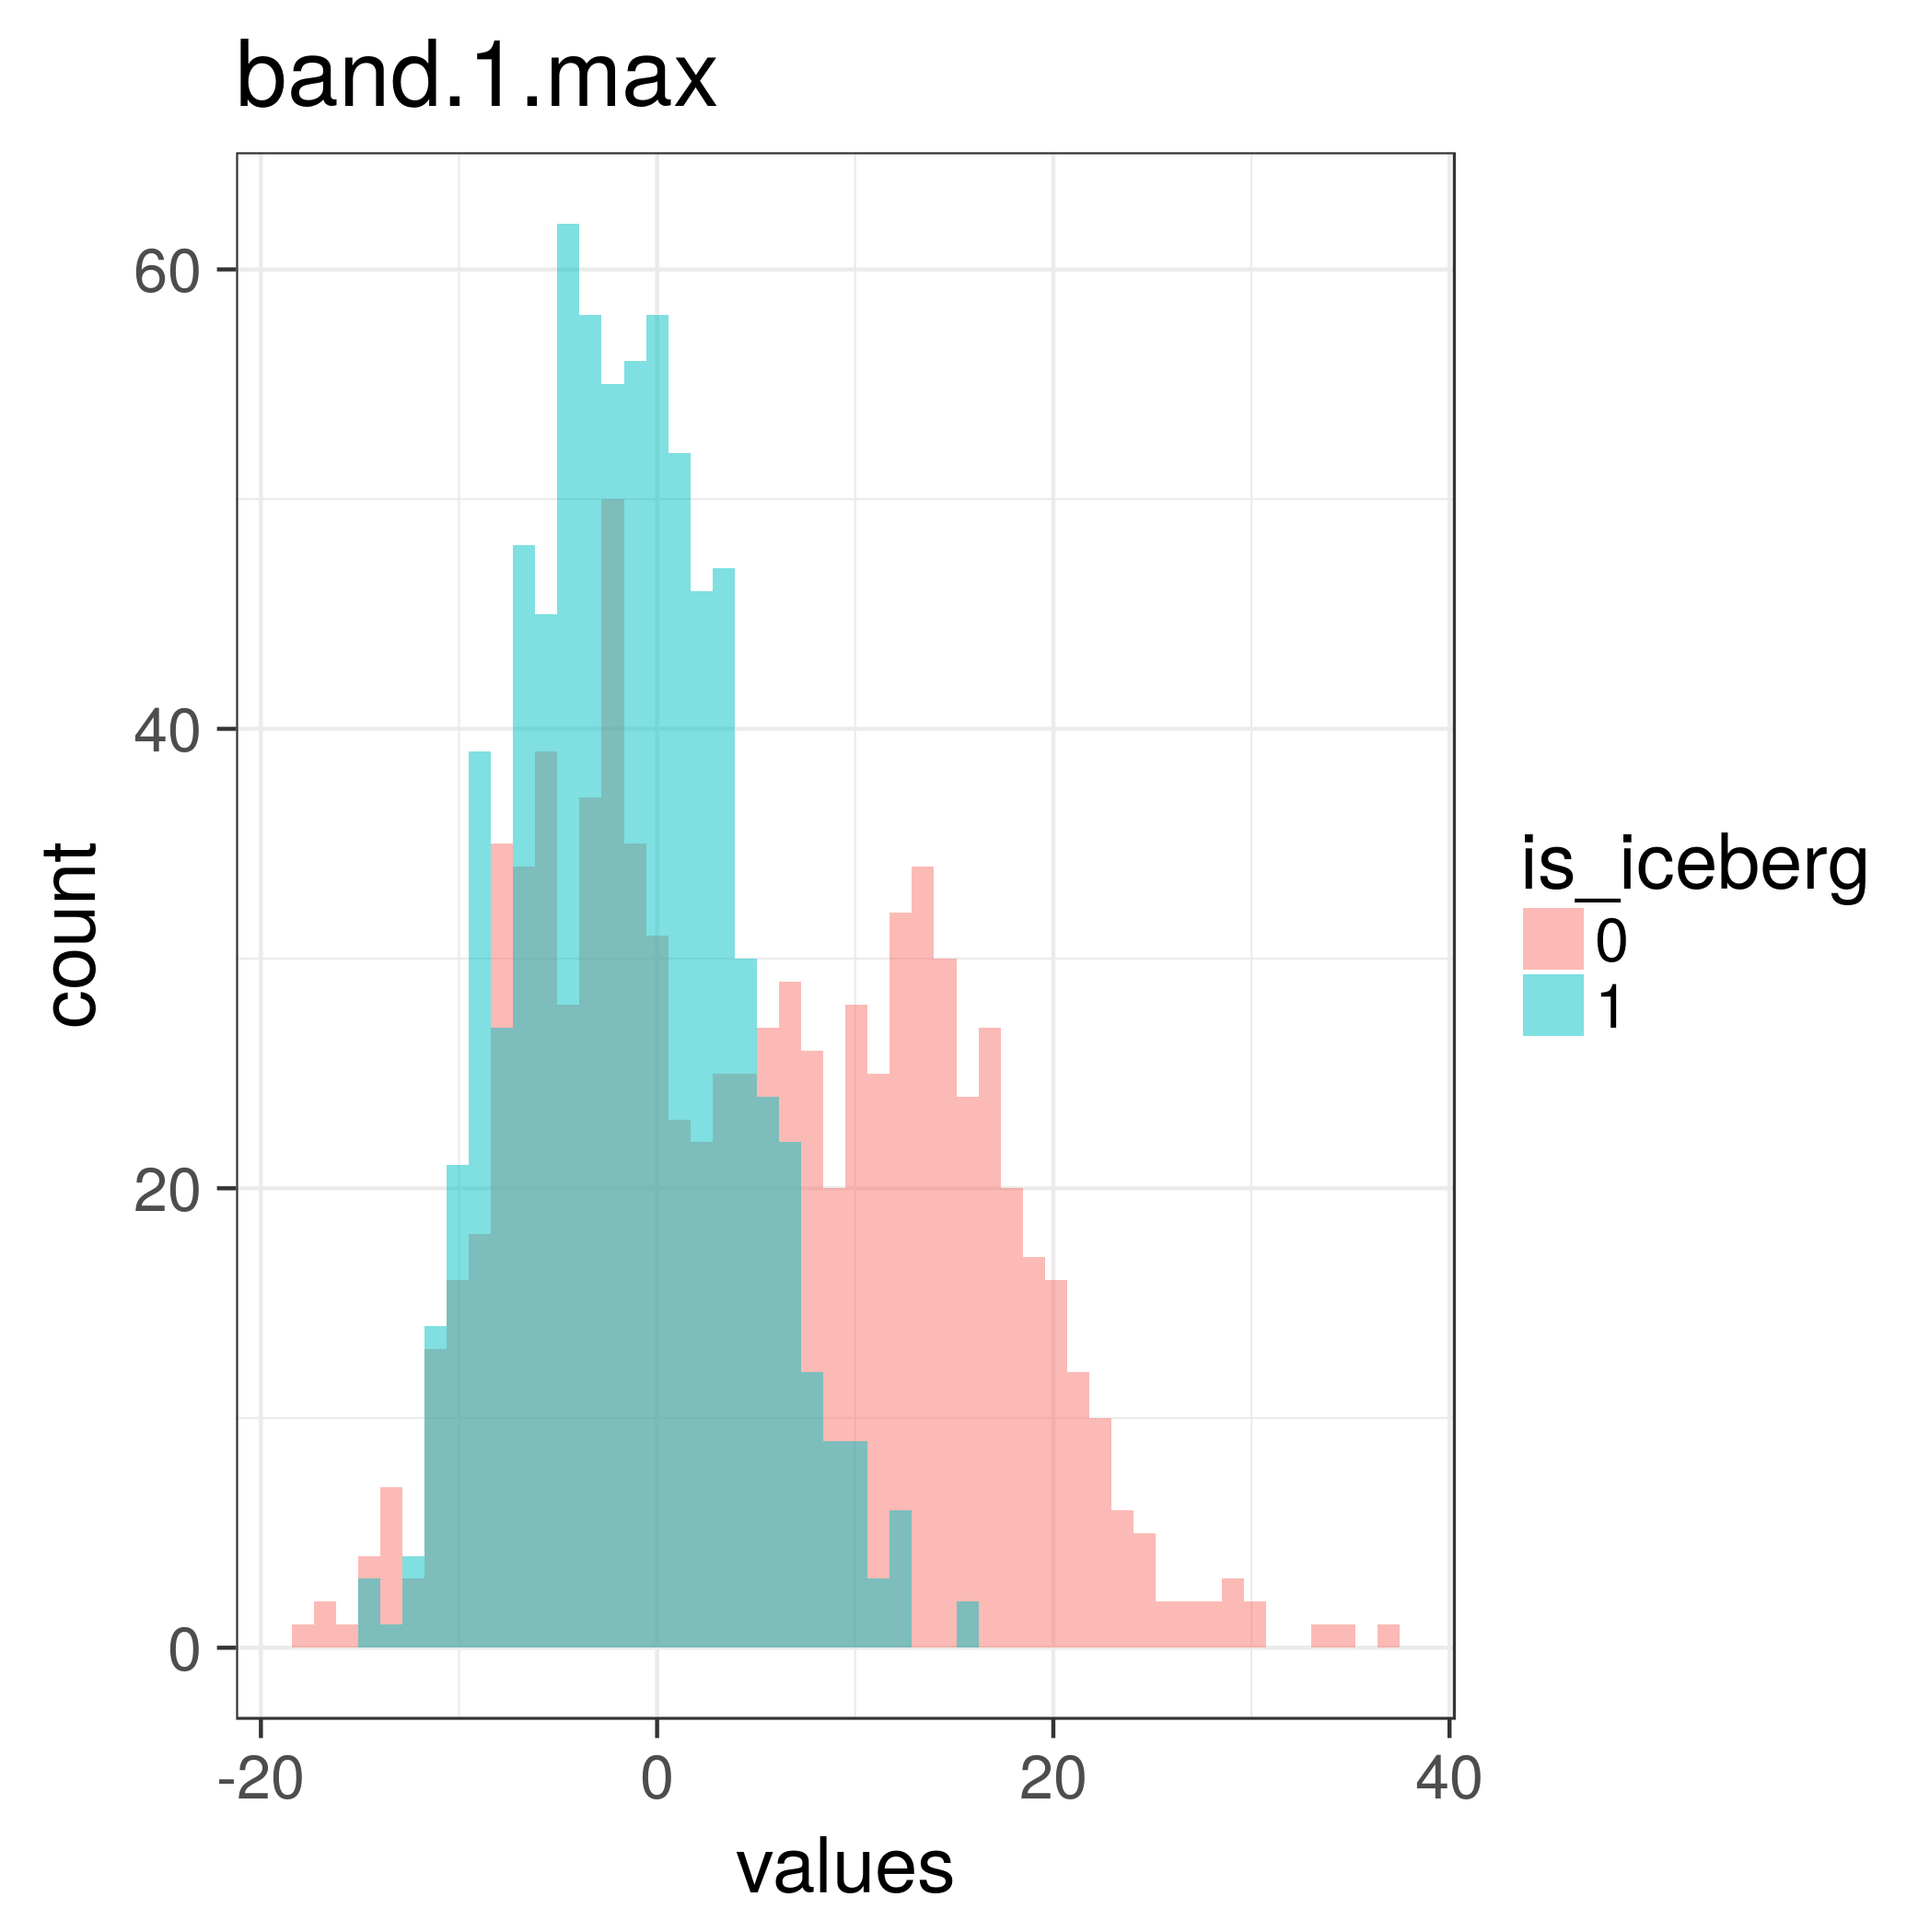
\includegraphics[scale=0.2]{iceberg/analysis/band_1_max.png}
	\end{minipage}%
	\begin{minipage}{0.24\textwidth}
		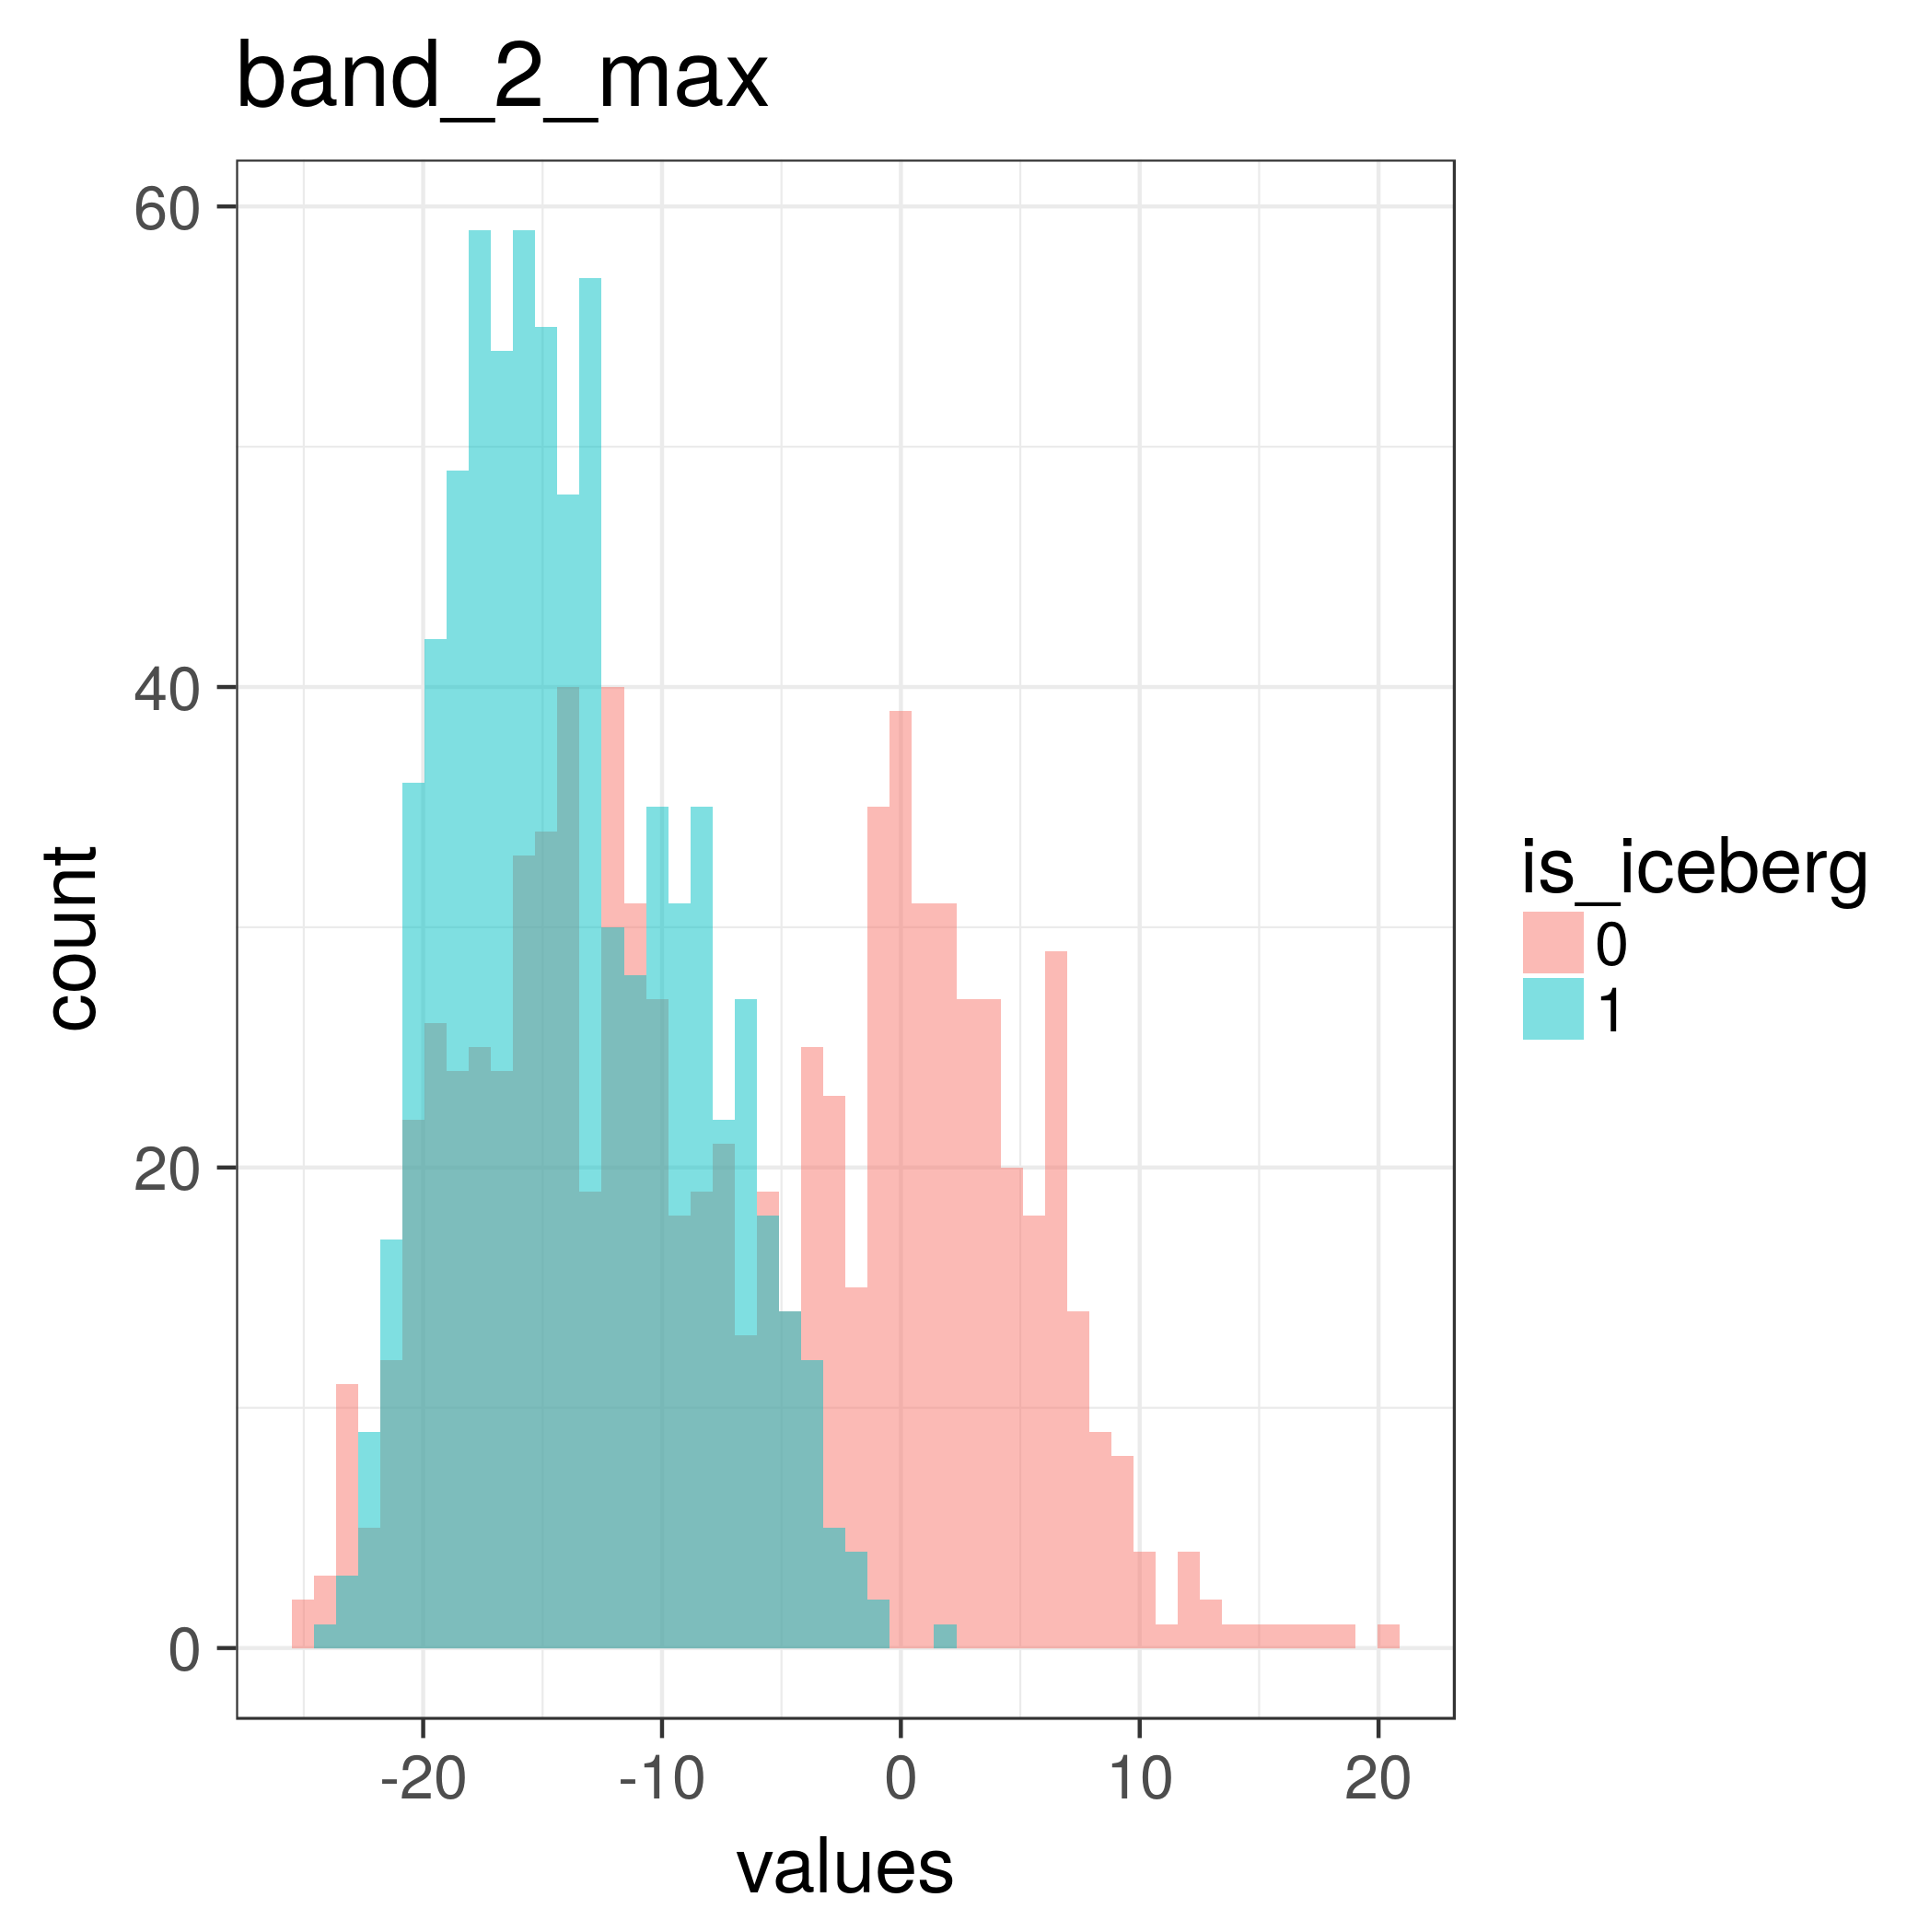
\includegraphics[scale=0.2]{iceberg/analysis/band_2_max.png}
	\end{minipage}
	\begin{minipage}{0.24\textwidth}
		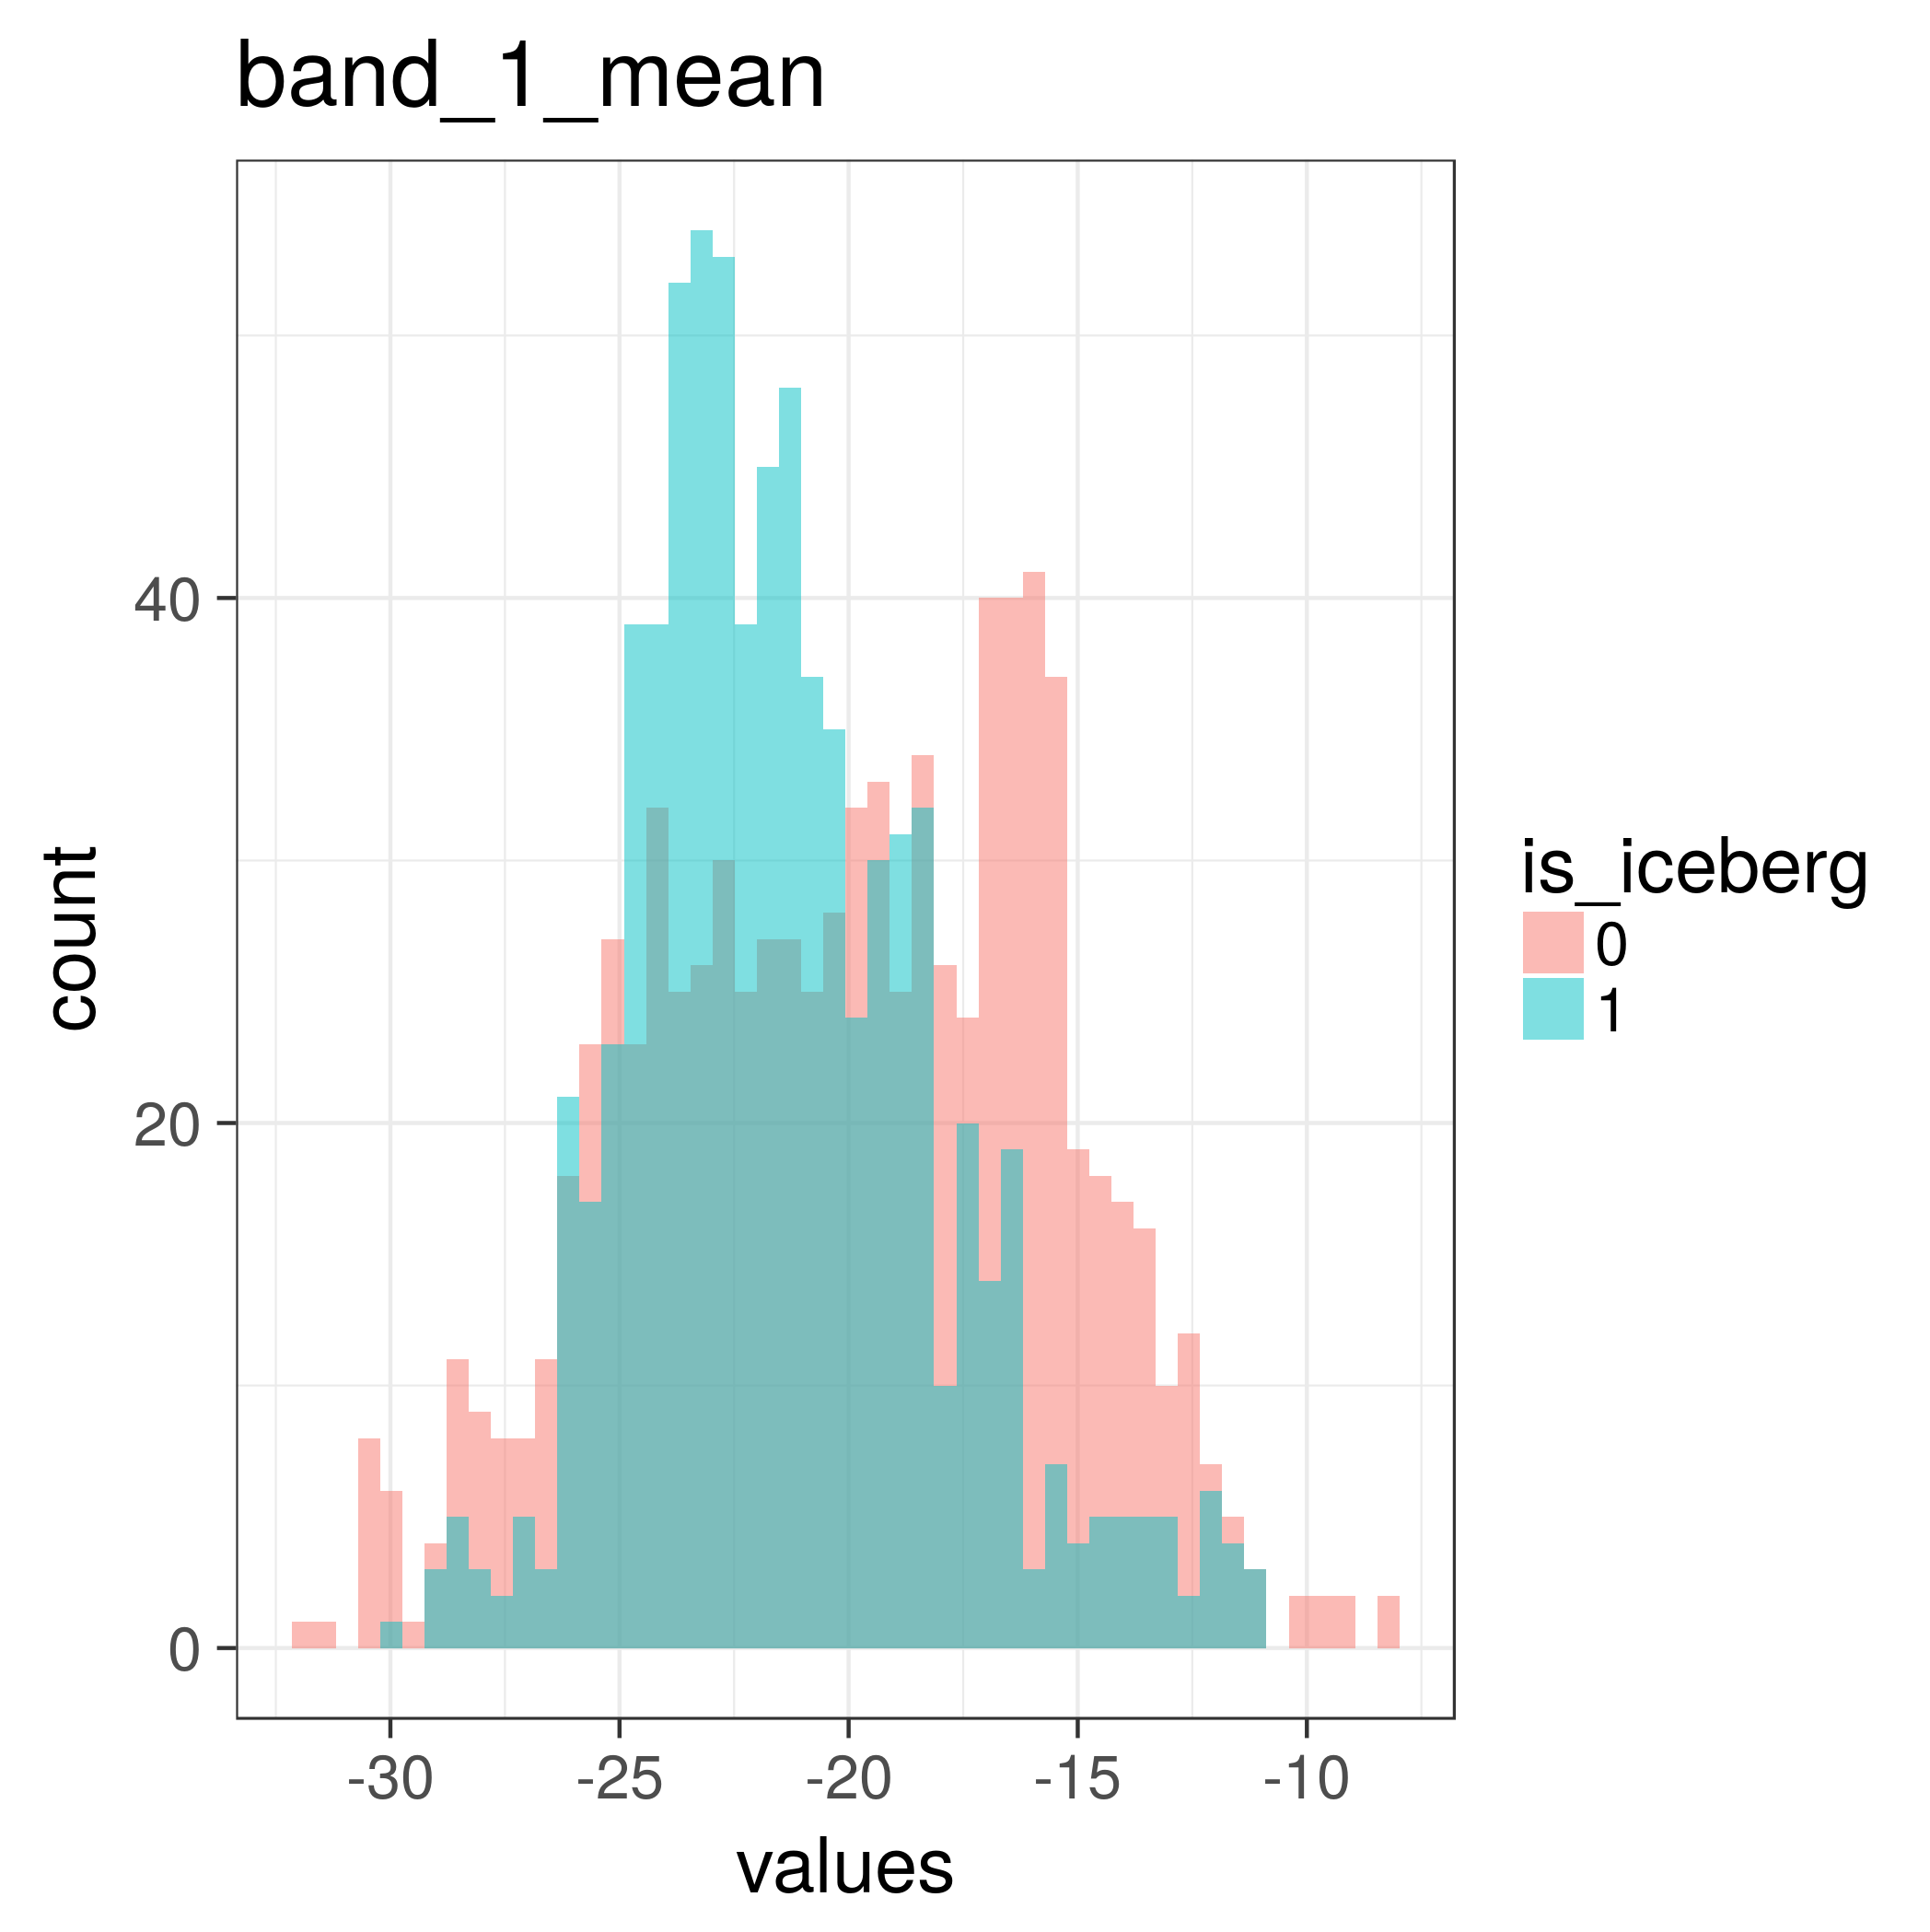
\includegraphics[scale=0.2]{iceberg/analysis/band_1_mean.png}
	\end{minipage}%
	\begin{minipage}{0.24\textwidth}
		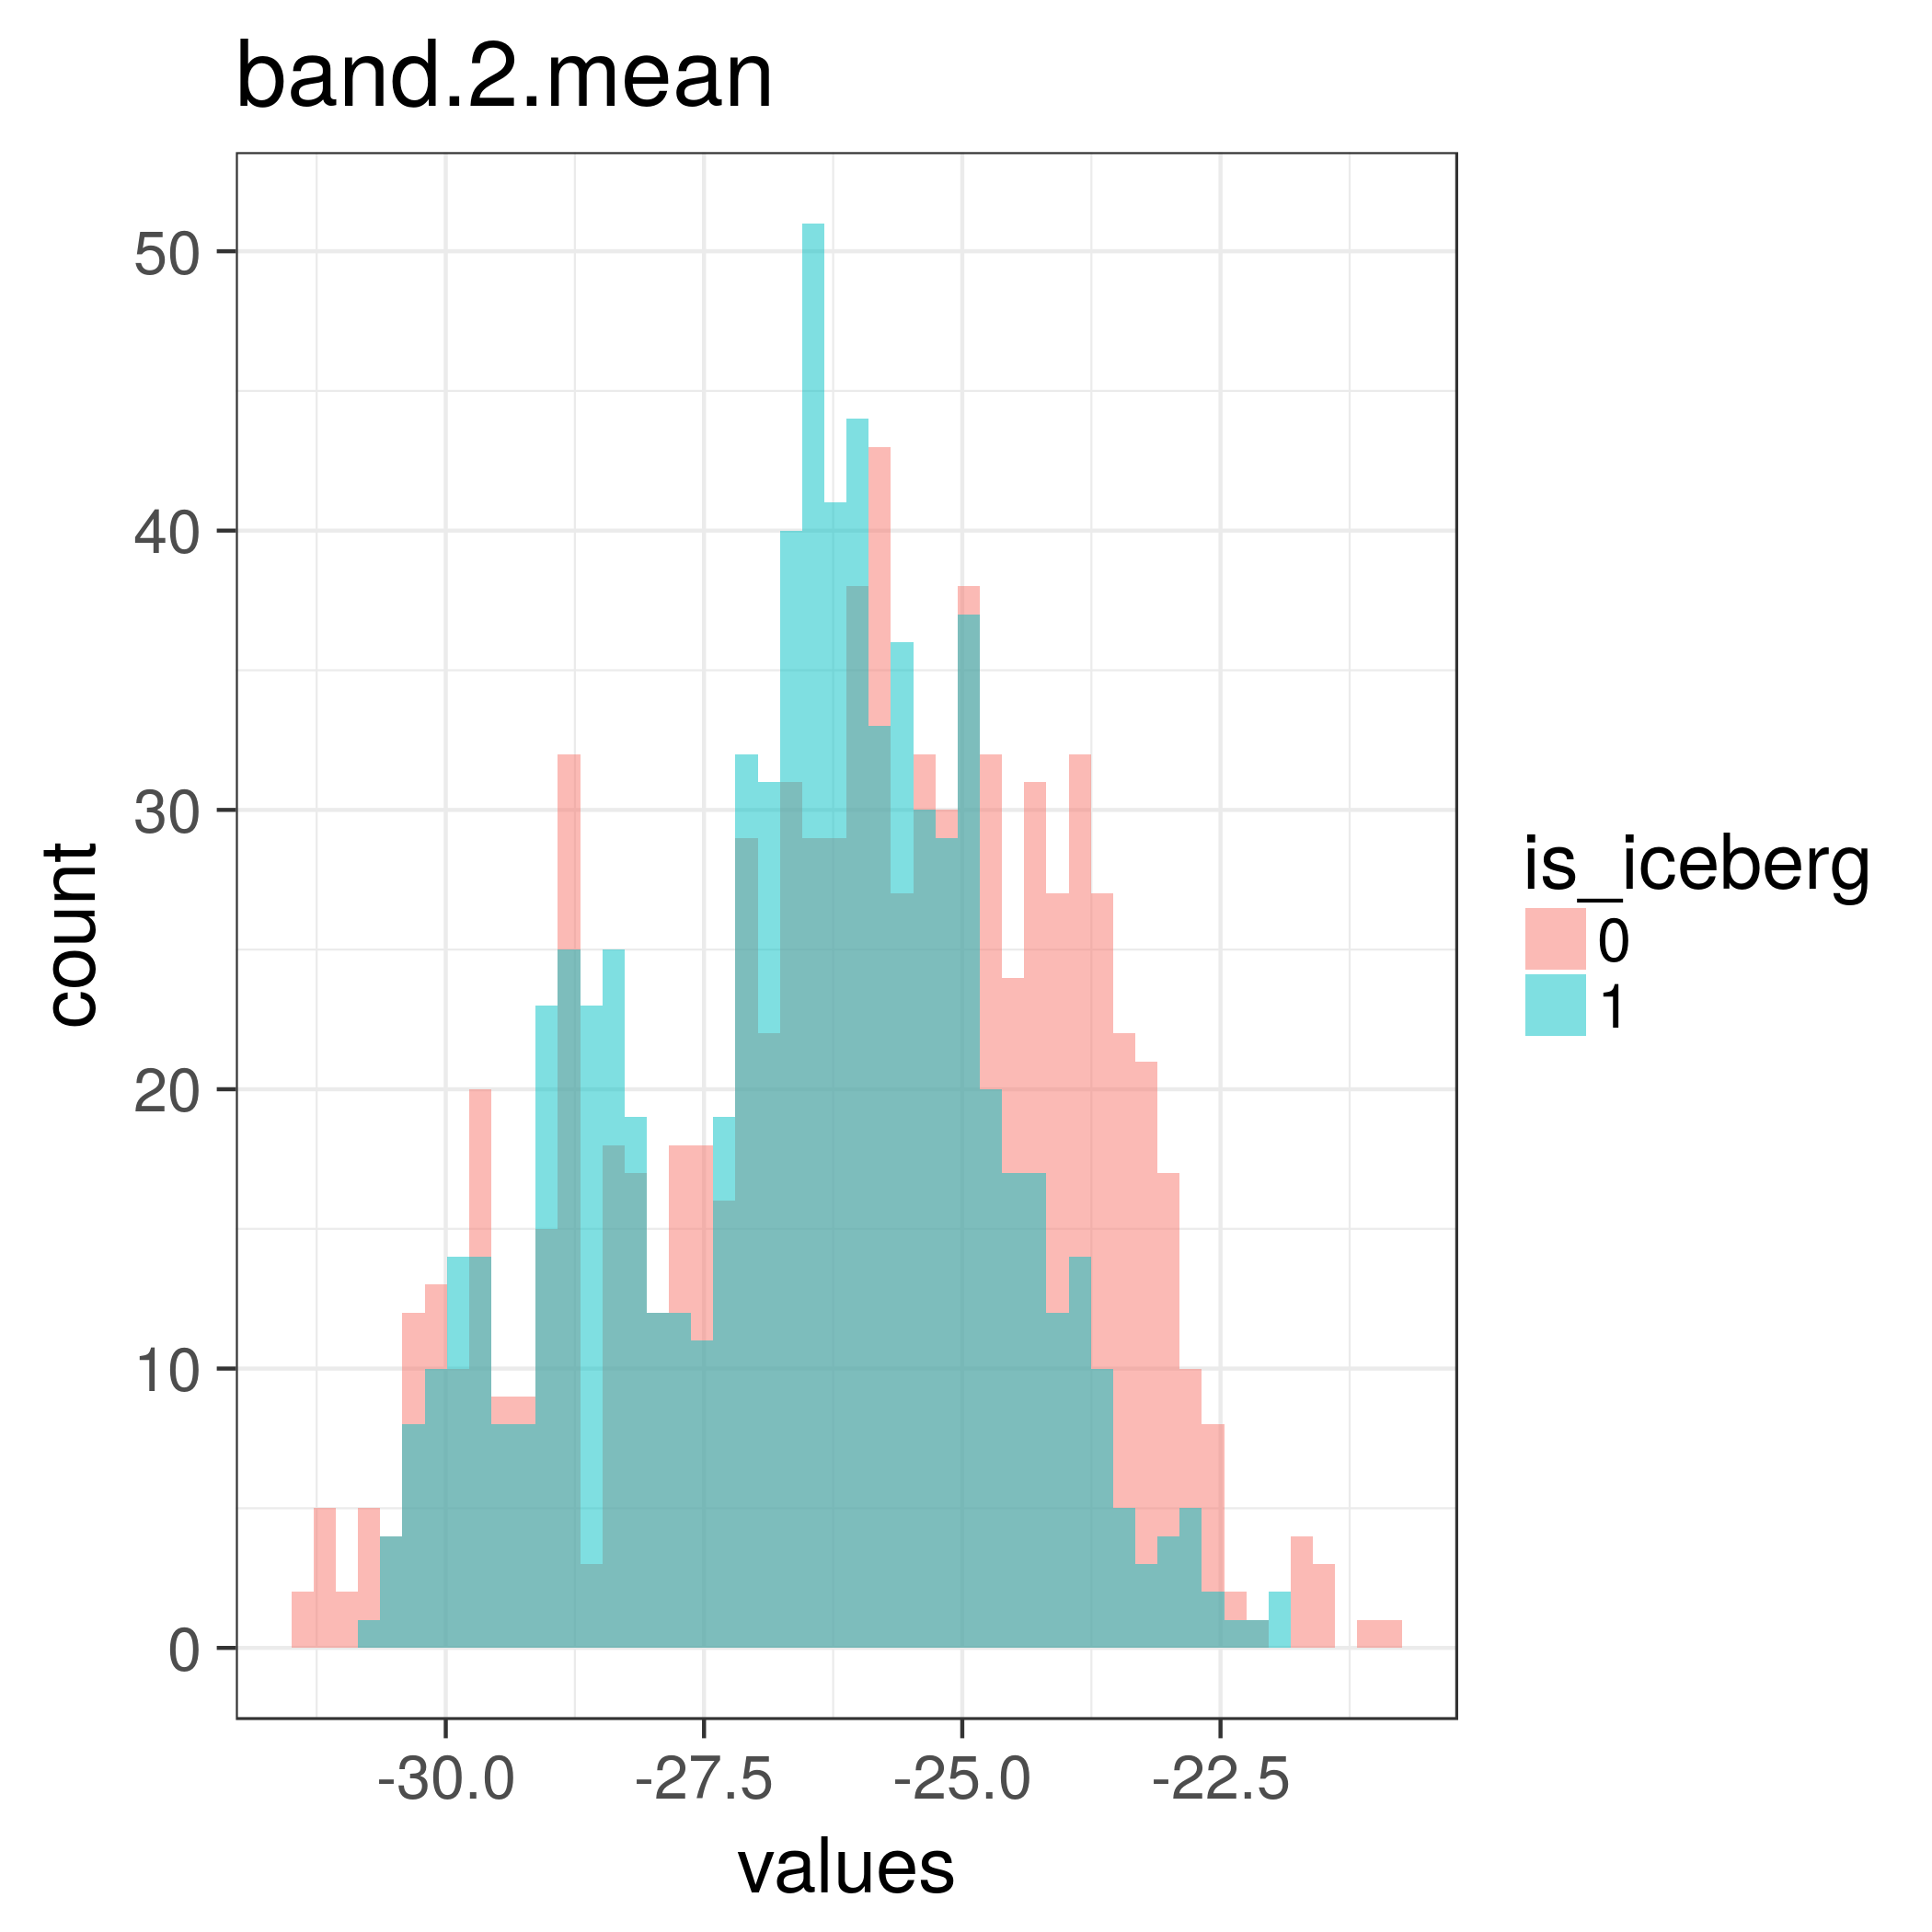
\includegraphics[scale=0.2]{iceberg/analysis/band_2_mean.png}
	\end{minipage}
	\caption{Band 1 and 2 Max and Mean}\label{max-mean-separable}
\end{figure}

\paragraph{Further Analysis} The overlap areas in the histograms represent those records that will cause difficulty for a classification model. Additional features are required for good performance.  The following functionality was developed to enable visual analysis as well as experimentation with new useful features:

\begin{itemize}
	\item Incidence angle has a perceived impact on backscatter intensity; see Figure \ref{inc_angle1}.  In this approach, simple linear regression was used to fit a line to background intensity as a function of incidence angle.  The intercepts for this line were used to normalize all the images to the mean incidence angle.  Those images whose incidence angle were not defined (NA) were not altered (i.e. assumed to have mean incidence angle).  The adjusted data is shown in Figure \ref{inc_angle2}.
	
	\item Simple convolution matrix filtering was implemented to achieve some rudimentary image processing.  Specifically, 3$\times$3 kernels were used for smoothing, sharpening, edge detection, and gradient. \cite{polarimetric} These filters were used to automatically produce images during visual analysis to aid in new feature development.  Examples are shown in Figure \ref{filtering}.  Notably, the plots for band 2 indicate potential higher-mode dependency, but that was not explored further.
	
	\item A simple center-finding function was implemented to calculate the sum of a sliding window over the image, and the position which yields the largest sum is taken to be centered on the object of interest (OoI).  Several of the features are calculated solely from a fixed-size mini-matrix centered on that position.  That mini-matrix is herein referred to as the `target'.  The intent was yield feature values that are more influenced by target pixels than by non-target pixels.
	
	\item TBD (Ashay, please talk about your HOG features here)
\end{itemize}

\begin{figure}\centering
	\begin{minipage}{0.45\linewidth}
		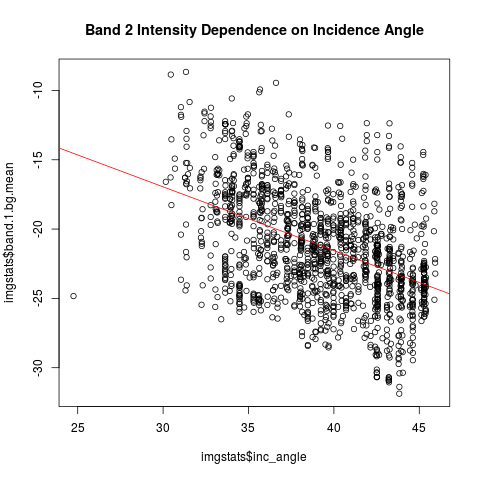
\includegraphics[width=.9\linewidth]{iceberg/analysis/b1_bg_intensity-ing_angle_prenorm.png}
	\end{minipage}%
	\begin{minipage}{0.45\linewidth}
		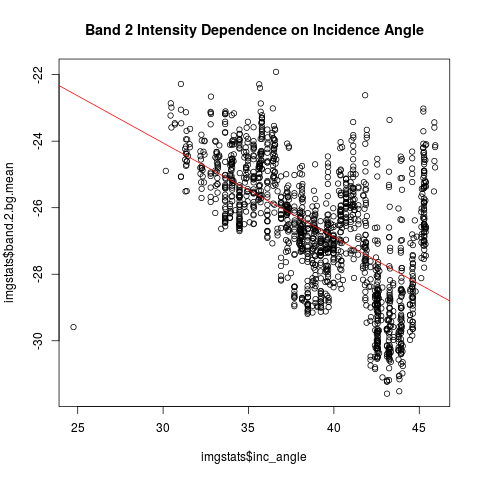
\includegraphics[width=.9\linewidth]{iceberg/analysis/b2_bg_intensity-ing_angle_prenorm.png}
	\end{minipage}
	\caption{Intensity Dependence on Incidence Angle}\label{inc_angle1}
\end{figure}

\begin{figure}\centering
	\begin{minipage}{0.45\linewidth}
		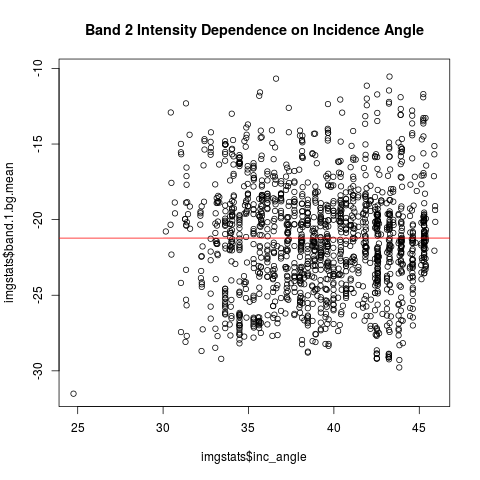
\includegraphics[width=.9\linewidth]{iceberg/analysis/b1_bg_intensity-ing_angle.png}
	\end{minipage}%
	\begin{minipage}{0.45\linewidth}
		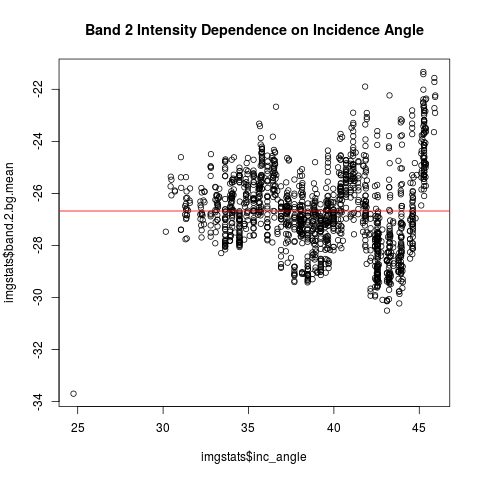
\includegraphics[width=.9\linewidth]{iceberg/analysis/b2_bg_intensity-ing_angle.png}
	\end{minipage}
	\caption{Normalized Intensity}\label{inc_angle2}
\end{figure}

\begin{figure}\centering
	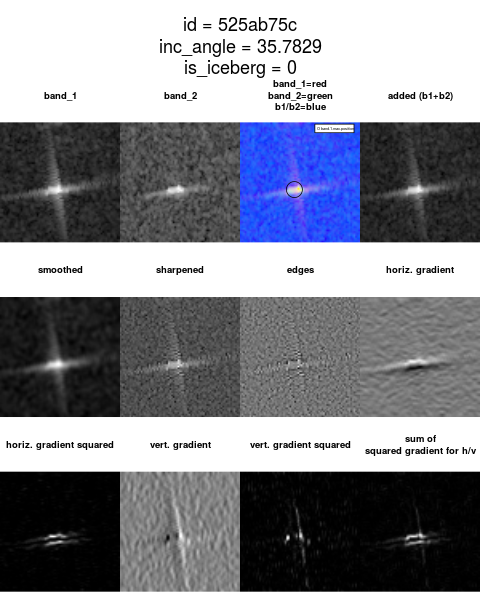
\includegraphics[width=.9\linewidth]{iceberg/analysis/525ab75c.png}
	\caption{Image Filtering}\label{filtering}
\end{figure}

\paragraph{Hypotheses} From visual analysis and research in the domain area \cite{wesche} \cite{Ship-Iceberg_CNN} \cite{howell}, several hypotheses were developed which drove new feature experimentation.

\begin{itemize}
	\item Ships are relatively sharp and angular, whereas icebergs are smooth and irregular, so differences in surface backscatter intensities (mean, max, variance) may yield class information.
	\item Volume backscatter properties of ice and metal \cite{howell} are different, so comparisons between band 1 and band 2 may yield some class information.  
	\item Icebergs (being made of frozen water) may have some observable characteristics that are similar to the surrounding water, whereas ships may not.  Therefore, comparison of the OoI to the background seawater may yield class information.
	\item The fast majority of iceberg volume is below the ocean's surface, and the angle of the ice as it protrudes from the water's surface is likely to be off-normal, whereas that of ships is likely to be near-normal.  Therefore, gradient and edge-detection approaches near the object-to-ocean transition area may yield class information.
	\item Incident angle is likely to have an effect on both the intensity and polarity of the return signal. \cite{makynen}
	\item TBD (Ashay, please talk about your hypotheses related to HOG features and how you predict they will enable classification)
\end{itemize}

\subsection{Methods}

\paragraph{Model Selection} Several classification methodologies were considered for this classification task: Convolution Neural Networks (CNN), Logistic Regression (LgR), TBD (Ashay), TBD (Ashay).  CNN methods have been shown to exhibit good performance on image recognition tasks. \cite{NIPS2012_4824} \cite{behnke}  Two challenges with Neural Networks are that (a) the more naive examples tend towards high-complexity and so require large data sets to achieve high accuracy and low variance, and (b) the hidden nature of the internal neurons pose challenges to applying useful domain knowledge to the classification problem.  They work particularly well in applications where they learn telling features of a visible object within the hidden layers.  In the context of this task, the size, shape, and orientation of the OoI is not believed to be as consistent and would be difficult to normalize, which would be highly desirable for a CNN approach.  CNNs, therefore, were not implemented. \cite{lecun}

LgR can be thought of as a special case of a Neural Network which has a single neuron that uses a logit function as its output.  The Since the single neuron is at the outer layer, its inputs and outputs are known.  This makes it straightforward to apply some domain knowledge to the raw data in order to provide inputs (features) that are thought to contain class information.  Additionally, the low complexity of the model makes it ideal for smaller training sets, such as the one provided by Kaggle. \cite{mccullagh} \cite{lim} The Logistic Regression Algorithm is shown in Algorithm \ref{alg:1}.  For this project, the authors used R's built-in \texttt{glm} function.

\paragraph{Logistic Regression} Essentially, LgR uses an initial guess of feature weights to transform the data feature vector into a value between 0 and 1, representing the probabilities that each record belongs to class 1.  A likelihood function and its derivative (with respect to the weights) are calculated, representing the curve of the likelihood that the weights are optimal over the domain of W.  The derivative use used to influence the magnitude and direction for which the weight vector should be adjusted.  The user-defined value $\alpha$ is also used to influence the step size of these adjustments.  This processes is repeated until the gradient is sufficiently small, representing the peak (or valley) of the likelihood function, indicating an optimal weight vector has been reached.

\begin{algorithm}
	\caption{Logistic Regression}
	\label{alg:2}
	\begin{algorithmic}[1]
		\STATE{\ {\bf INPUT:} data $X_{n \times (d-1)}$, class labels $C_{n \times 1}$ }
		\STATE{\ {\bf OUTPUT:} weights $W_{1 \times d}$ }
		\STATE \%\% Define gradient descent parameters
		\STATE{\ $\epsilon \leftarrow$ user threshold }
		\STATE{\ $\alpha \leftarrow$ user step size }
		\STATE \%\% Add ones column for offset
		\STATE{\ $X \leftarrow \left[ X_{n \times (d-1)} \vec{1}_{n \times 1} \right] $ }
		\STATE \%\% Initialize weights
		\STATE{\ $W \leftarrow \vec{0}_{d \times 1}$ } 
		\WHILE { $\left| \nabla_W L(W) \right| > \epsilon$ }
		\STATE \%\% Class probability as function of weights
		\STATE{\ $y_i(W) \leftarrow \frac{1}{1 + e^{-x_iW}} \forall x_i \in X$ }
		\STATE \%\% Likelihood as function of weights
		\STATE{\ $L(W) \leftarrow -\sum_{i=1}^{n} c_i log(y_i) + (1-c_i) log(1-y_i)$ }
		\STATE \%\% Gradient of likelihood wrt weight vectors
		\STATE{\ $\nabla_W L(W) \leftarrow \sum_{i=1}^n x_i (y_i - c_i)$ }
		\STATE \%\% Update weights
		\STATE{\ $W \leftarrow W + \alpha \nabla_W L(W)$ }
		\ENDWHILE
		\RETURN $W$
	\end{algorithmic}
\end{algorithm}

\paragraph{TBD}
TBD (Ashay, briefly describe your modeling approach for each algorithm)

\paragraph{Features} The LgR modeling approach enabled experimentation of new potential features, which became the next focus.  Table \ref{more-features} summarizes, in some detail, a few of the more interesting features that were explored for LgR based on the previously mentioned visual analysis and domain research.  Additional features are briefly described below.

\begin{table*}[ht]
	\caption{Additional Features for LgR}\label{more-features}
	\begin{tabular}{l p{.45\linewidth} l}
		\toprule
		Feature & Description & Histogram \\
		\hline \vspace{10pt} \\
		\rotatebox[origin=r]{90}{\texttt{tar.sum.gs.sum.mean}} &
			The target mini-matrix for each band is added together.  The result is filtered by vertical gradient and horizontal gradient kernel in parallel. Those two results are then squared and added together, and the mean of the result is taken to be the new feature.  The intent of this feature is to let both bands contribute to squared gradient result.  Two theories are at work here: (a) The edges of ships are vertical and so one might expect a sharper ship-to-water transition, resulting in a higher gradient, and (b) since icebergs are more similar in texture and composition to water than are ships, that may also contibute to a sharper contrast between ship and water, again resulting in a higher gradient. &
			\begin{minipage}[t]{0.35\linewidth}
				\adjustimage{width=1\linewidth,valign=t}{iceberg/analysis/tar_sum_gs_sum_mean.png}
			\end{minipage}\\%
		\rotatebox[origin=r]{90}{\texttt{tb.mean.dif.dif}} & 
			Visual analysis revealed most images to be rather centered on the OoI.  A fixed-size border mask (think picture frame) was created to provide the subset of pixels presumed to reside in the background.  For each band, the background mean was subtracted from the target mean.  The restult for band 2 was then subtracted from the result for band 1, and the final result was taken to be the feature.  The intent was essentially to see if the difference in target-to-background contrast between bands may contribute to classification.  Put another way, the depolarizing properties of ice may be similar to that of the surrounding water, creating a consistently lower contrast image in band 2 as compared with band 1 for icerbergs. &
			\begin{minipage}[t]{0.35\linewidth}%\centering
				\adjustimage{width=1\linewidth,valign=t}{iceberg/analysis/tb_mean_dif_dif.png}
			\end{minipage}\\%
		\rotatebox[origin=r]{90}{\texttt{tar.cor}} & 
			The band 1 and band 2 images are first smoothed to reduce extreme values caused by noise or speckle and zero-adjusted.  Next, all of the pixel values that are greater than 0.7 of the maximum value are kept, the others discarded.  These pixels are then used as a mask to extract all of the pixels in the raw image which are presumed to belong to the OoI.  Finally, a correlation is calculated between these pixels between band 1 and band 2, and the resulting value is taken to be the feature.  The intent is to capture how well band 2 correlates to band 1 over the OoI.  The theory is that depolarization effect would affect correlation and be different for icebergs than for ships. &
			\begin{minipage}[t]{0.35\linewidth}%\centering
				\adjustimage{width=1\linewidth,valign=t}{iceberg/analysis/tar_cor.png}
			\end{minipage}%
	\end{tabular}
\end{table*}

\begin{itemize}
	\item{\textbf{\texttt{band.1/2.tar.var}}} Variation of image pixels in the target for each band.  The seed for this idea originated from Bentes \cite{Ship-Iceberg_CNN} who recognized variance among other signal characteristics as harmful in a Neural Network approach and therefore something to be reduced.  The intent is to see whether there is class information found within the variance of the return signal from the target.
	\item{\textbf{\texttt{band.1/2.tb.mean.dif}}} The difference of means of the target and border regions of the image pixels for each band.  The intent is to see if there is class information derivable from return signal intensity from the target as compared with the background.
	\item{\textbf{\texttt{band.1/2.tar.gvs.mean}}} The target in each band was filtered using a vertical gradient filter and then squared, and the mean of the result was taken for each band.  The intent is to see if there is class information in the object-to-ocean interface area that would be captured by the gradient filter.
	\item{\textbf{\texttt{band.1/2.tar.ghs.mean}}} The target in each band was put through a horizontal gradient filter and then squared, and the mean of the result was taken for each band.
	\item{\textbf{\texttt{band.1/2.tar.mean}}} A mean was taken of the target pixels for each band.
	\item{\textbf{\texttt{tar.gvs.dif}}} The target in each band was filtered using a vertical gradient filter, squared, and meaned.  The result from band 2 was subtracted from that of band 1.
	\item{\textbf{\texttt{tar.ghs.dif}}} The target in each band was filtered using a horizontal gradient filter, squared, and meaned.  The results from band 2 was subtracted from that of band 1.
\end{itemize}

\paragraph{Challenges} Some challenges and drawbacks to the chosen modeling approaches include the following.

\paragraph{}Logistic Regression:
\begin{itemize}
	\item{Structure Simplicity:} LgR is capable of creating arbitarily complex models based on the number input features.  However, as a statistical tool, it lacks some of the structural features of other models such as decision trees and neural nets.  Because of this, the LgR model alone is not capable of branching on specific features.
	\item{Feature Selection:} During experimentation with new and existing feature, simple histogram analysis revealed many of the candidate features as containing some class information (i.e. good separability of classes over the feature).  However, pairs of features are highly correlated and others were not (See figure \ref{correlation}).  It is difficult to choose which features to include manually.
\end{itemize}

\begin{figure}
	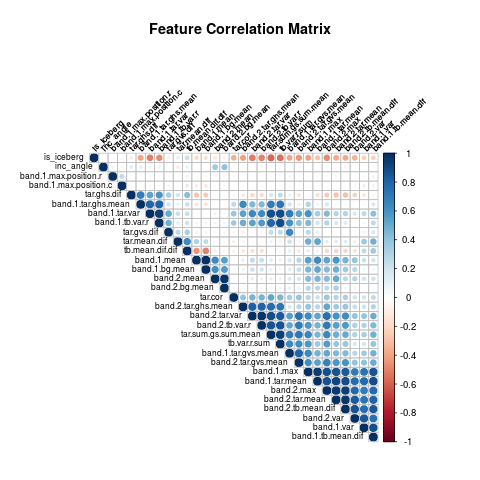
\includegraphics[width=.9\linewidth]{iceberg/analysis/corr_matrix.png}
	\caption{LgR Feature Correlation}\label{correlation}
\end{figure}

\paragraph{}TBD (Ashay, describe challenges with your approaches)

\paragraph{Implementation} 
\paragraph{}Lgr - Given the manual nature of the feature development and experimentation approach chosen, it was important to automate updates to the analysis, training, and validation approach to the greatest extent possible.  Automation of these aspect enables rapid identification and incorporation of improvements to the feature set.  To this end, all database interaction, image processing, and feature calculation was centralized to a single code source.  An analysis script was run after each change to the feature set to quickly visualize some characteristics of new features.  In addition to automation, V-fold cross validation was utilized as the primary means of model performance prediction.  It should be noted that test data used in cross-validation was present during all data analysis tasks, which may introduce bias as a result in the model selection process. \cite{cawley}  Finally, a simple greedy algorithm was chosen to select which features to use during the training process.  Essentially, starting from an empty feature set, the feature which (when added to the set) results in the lowest Log Loss on the test data during V-fold cross validation is added.  A subset of the (now ordered) feature list which results in the lowest total Log Loss on the test data is then selected for use.  The author notes this algorithm is not guaranteed to find the optimal set of features on which to train.  In fact it was observed that some of the later Kaggle submissions (which represented a superset of features as compared with past submissions) achieved worse performance!  This is because the optimal subset of features was never encountered during the greedy selection process.

\begin{algorithm}
	\caption{LgR Feature Selection}
	\label{alg:3}
	\begin{algorithmic}[1]
		\STATE{\ \textbf{Def:} $ vFoldXVal(\Delta \left[ features \right] ) \rightarrow LogLoss_{test}$ }
		\STATE{\ {\bf INPUT:} feature list $F$, labeled data $\Delta$ }
		\STATE{\ {\bf OUTPUT:} selected feature list $F_S$ }
		\STATE{\ $F_S \leftarrow \emptyset$ }
		\STATE{\ $F_S.last \leftarrow $ NA }
		\STATE{\ $F_S.lossmin \leftarrow \infty$ }
		\WHILE{\ $F \neq \emptyset$ }
		\STATE{\ $f_{best} \leftarrow$ NA }
		\STATE{\ $f_{best}.loss \leftarrow \infty$}
		\FOR{\ $f$ in $F$}
		\STATE{\ $loss \leftarrow vFoldXVal(\Delta\left[\{F_S\} \cup \{f\} \right])$ }
		\IF{\ $loss < f_{best}.loss$ }
		\STATE{\ $f_{best} \leftarrow f$ }
		\STATE{\ $f_{best}.loss \leftarrow loss$ }
		\IF{\ $loss < F_S.lossmin$ }
		\STATE{\ $F_S.last \leftarrow f$ }
		\STATE{\ $F_S.lossmin \leftarrow loss$ }
		\ENDIF
		\ENDIF
		\ENDFOR
		\STATE{\ $F_S \leftarrow \{F_S\} \cup \{f_{best}\}$ }
		\STATE{\ $F \leftarrow F \setminus \{f_{best}\}$ }
		\ENDWHILE
		\STATE{\ $F_S \leftarrow F_S\left[1:F_S.last\right]$ }
		\RETURN $F_S$
	\end{algorithmic}
\end{algorithm}

\paragraph{}TBD (Ashay, describe your implementations for each algorithm)

\subsection{Results}

\paragraph{Processing Performance}
Feature calculation, model training and feature selection, and classification were performed on a personal laptop, the specifications of which are found in Table \ref{machine-specs}.  Processing times are shown in Table \ref{proc-time}.

\begin{table}[H]
	\centering
	\caption{Machine Specifications for LgR}\label{machine-specs}
	\begin{tabular}{r l}
		\toprule
		\textbf{Processor:} 		& Intel Core i5-5200 @ 2.2 GHz x 4 \\
		\textbf{Memory:}			& 8 GiB \\
		\textbf{Operating System:}	& Ubuntu 16.04 LTS \\
		\textbf{Applications:}		& R and MySQL \\
		\textbf{R Packages:}		& RMySQL, rjson, grid, ggplot2, \\
									& corrplot
	\end{tabular}
\end{table}

\begin{table}[H]
	\centering
	\caption{Processing Time (mm:ss) for LgR}\label{proc-time}
	\begin{tabular}{r l}
		\toprule
		\textbf{Feature Calculation:} 		& 02:22 \\
		\textbf{Feature Selection:}			& 01:26 \\
		\textbf{Model Training:}			& 00:00  \\
		\textbf{Test Data Classification:}	& 13:04 \\
		\textbf{Total:}						& 16:52
	\end{tabular}
\end{table}

TBD (Ashay, put your machine specs and processing time here)



\paragraph{LgR Feature Selection Performance}
One might assume that the feature selection ordering may well correlate well with those chosen by visual examination of the histograms, but that is not the case.  Since some of the features inform on some of the others, once a feature is selected and incorporated into the model, the addition of a feature that is highly correlated to one already in the set would result in little performance improvement.  The performance of the LgR model as a function of features added is shown in Figure \ref{feat_selection}.  Overall, the performance on test data tracks relatively well to performance on training data, suggesting that overfitting is not occuring to a great extent for the first dozen or so features.

\begin{figure}
	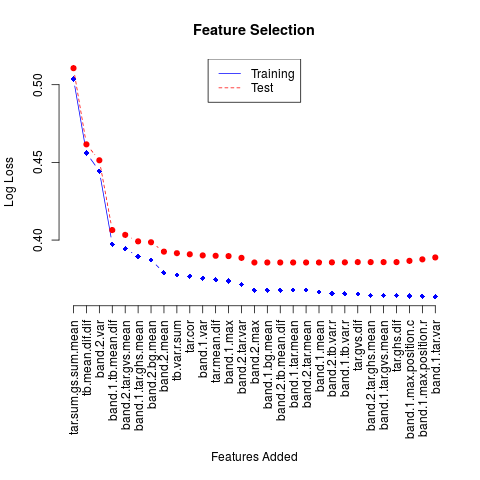
\includegraphics[width=.9\linewidth]{iceberg/feat_sel.png}
	\caption{Performance During Feature Selection for LgR}\label{feat_selection}
\end{figure}

\paragraph{Predictive Performance}
LgR - The best performance achieved as of the writing of this paper is \textbf{0.3682}, which is about the 18th percentile as of the submission of this paper. \footnote{Kaggle's scoring script uses Log Loss, which is consistent with the evaluation methods used herein}.  The Receiver Operator Characteristics (ROC) plot is shown in Figure \ref{roc}.

\begin{figure}
	\centering
	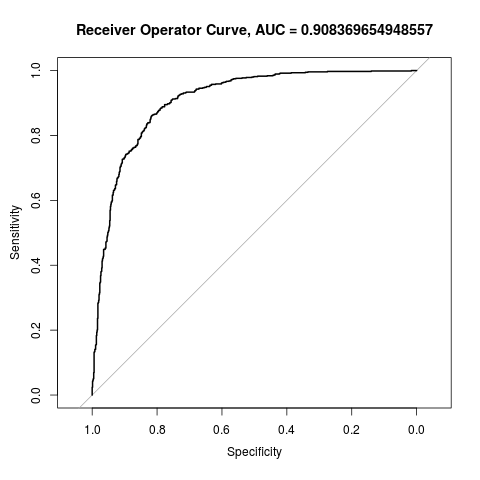
\includegraphics[width=0.9\linewidth]{iceberg/ROC_Results.png}
	\caption{Logistic Regression ROC Results}\label{roc}
	\small
	Sensitivity represents icebergs correctly classified as icebergs, and specificity represents non-icebergs incorrectly classified as icebergs.
\end{figure}

TBD (Ashay, please talk about your performance here)

\subsection{Summary and Future Work}
\paragraph{Summary}
The performance of the LgR classifier resulting from this effort was not exemplary.  The methodology chosen for feature experimentation and calculation was manual and labor intensive, and frankly the problem is not within the author's domain of experience.  The author hypothesizes that the high level of mutual information shared by many of the custom features ultimately limited learning performance of the model.  This hypothesis is supported by both Figure \ref{correlation} and Figure \ref{feat_selection}.  The author considers the project a success, despite the average results achieved.  The lessons learned about how to plan and structure a DM project as well as some of the practical aspects of implementing algorithms and dealing with real data will serve the author well.

TBD (Ashay, elaborate/modify as needed)

\paragraph{Future Work}
Some potential future improvements to the LgR approach would be to adopt an entropy-based or correlation-based feature selection algorithm rather than the simple greedy algorithm described herein - that would enable the selection of features according to the information they contain about class, derived from their probability density functions or correlation to class label vs other existing features, respectively.  

Further, one could revisit the Neural Network approach which would allow for nonlinearity and higher complexity.  Neural Networks could incorporate both custom features (as described in the LgR approach) as well as image-oriented features such as the image processing filters discussed herein or the Histogram of Oriented Gradients.  Additionally, some additional domain expertise applied to this problem would surely result in more relevant features which capture more of the known physical phenomena related to SAR imagery that could impact classification performance.  The higher-mode behavior observed in the plots of background intensity as a function of incidence angle is just one example.

TBD (Ashay, any future work you've identified?)



%------------------------------------------------
\phantomsection
\section*{Acknowledgments} % The \section*{} command stops section numbering
The authors would like to thank our professor, Dr. Mehmet Dalkilic, for his superior guidance and quick wit in the classroom; our parents for their continued recognition that we have not yet achieved our full potential; and Indiana weather, which provided ceaseless encouragement to stay indoors and pursue Datamining greatness.
\addcontentsline{toc}{section}{Acknowledgments} % Adds this section to the table of contents



%----------------------------------------------------------------------------------------
%	REFERENCE LIST
%----------------------------------------------------------------------------------------
\phantomsection
\bibliographystyle{unsrt}
\bibliography{sample}

%----------------------------------------------------------------------------------------

\end{document}
